\section{Task 2: Reverse engineering the RF protocol} \label{ch:pentesting:rf-reverse-engineering}
This section covers the process of reverse engineering the RF protocol, via captured RF signals. This included mainly trying to demodulate the signals into binary data and then analyzing the contents.

\subsection{Background}
The system in question uses RF signals to wirelessly communicate across the devices. These radio waves are used to transfer binary data, ones and zeroes, between each device. Transferring binary data over radio waves is done by a process called modulation \cite{rf-modulation}. Digital modulation, e.g modulating binary data, is a whole field of study on to it self and that this is only a brief overview covering the basics of modulation.

There are three primary simple ways of modulating a binary signal: Amplitude- (ASK), Frequency- (FSK), and Phase- (PSK) shift keying. They each produce a distinct wave form, which can easily be visually identified. This is shown in figure \ref{fig:digital-modulation}.
\begin{figure}[!ht]
    % Perhaps I don't have the license to use this?
    \centering
    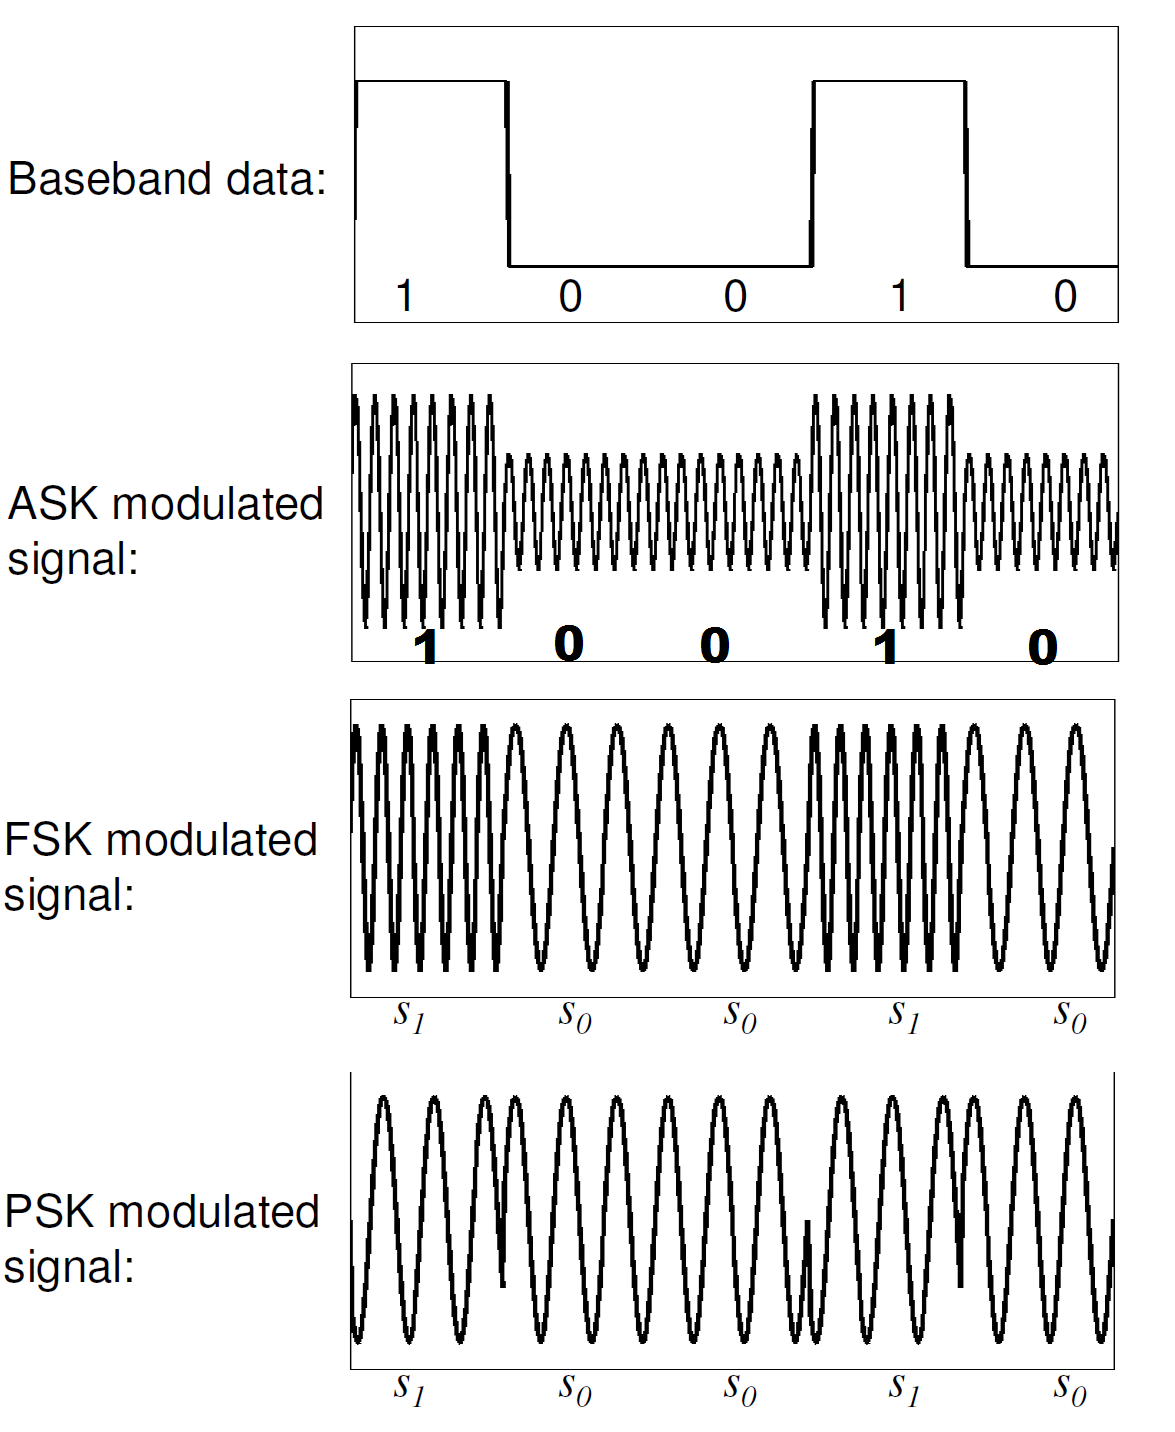
\includegraphics[width=0.7\textwidth]{images/6-pentesting/digital-modulation.png}
    \caption{The three primary techniques for digital modulation.}
    \label{fig:digital-modulation}
\end{figure}
Each technique uses a different property of the sinusoidal wave to encode a zero and one respectively. \gls{ASK} uses the amplitude of the wave, where a higher amplitude usually encodes a \texttt{1} and a lower amplitude a \texttt{0}. The frequency and phase of the wave is kept constant. \gls{FSK}, on the other hand, keeps both amplitude and phase constant. Instead two different frequencies are shifted between to differentiate between a \texttt{0} or \texttt{1}. Lastly, \gls{PSK} uses a phase-shift to differentiate between the two symbols. There are many much more complicated techniques to more efficiently encode a binary signal in radio waves \cite{rf-modulation}. However, these are not covered in this report.

Conversely, \textit{demodulation} is the process of covering a modulated signal back into the original binary data. In most real world applications of RF communication this is done directly in hardware, using specific radio receivers and circuitry to automatically convert the signal back into binary data \cite{rf-modulation}. Often this hardware also implements error correction and other techniques to increase reliability of the communication, as interference and other disturbances are unavoidable in the real world. Figure \ref{fig:bfsk-demodulator} shows a very simplified circuit that implements binary FSK (BFSK) demodulation, e.g FSK modulation using two parameter frequencies.
\begin{figure}[!ht]
    \centering
    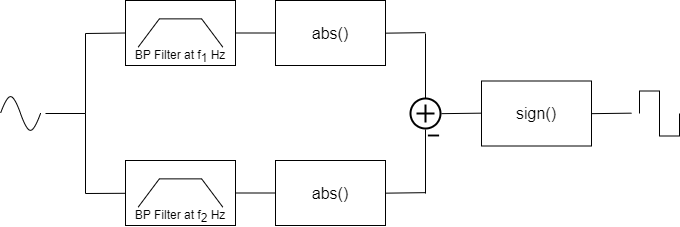
\includegraphics[width=\textwidth]{images/6-pentesting/bfsk-demodulator.png}
    \caption{A simplified BFSK demodulating circuit.}
    \label{fig:bfsk-demodulator}
\end{figure}
Given a BFSK signal, modulated using the frequencies $f_1$ and $f_2$, the circuit does the following. First the signal is split and passed into two band-pass filters, tuned to the two respective parameter frequencies. Then the absolute value is applied to the signals, one of them is inverted, and they are added together. Lastly, to convert the result into the final binary wave, the signal is passed to the $sign()$ function. This circuit was inspired by material from the course \textit{EE123 Digital Signal Processing} at Berkeley EECS, specifically Lab 4 which covers FSK demodulation\footnotelink{https://sites.google.com/berkeley.edu/ee123-sp20/labs}{2021-05-18}. Demodulation can of course also be done in software, but doing so in real-time is quite CPU-intensive and consequently a lot less energy efficient. Moreover, for each modulation type there are several tuneable parameters that are hard coded in the hardware demodulation chip, such as the frequencies of the FSK modulation, which during reverse engineering have to be figured out.

\subsection{Method}
Initially, signals were captured according to the method described in section \ref{ch:pentesting:replay:method}. Carefully inspecting the signals in \gls{URH}, as shown in figure \ref{fig:rf-signal-capture}, one can see that clearly \gls{FSK} modulation is used to modulate the signal. This conclusion is strengthened by official test documentation submitted to the \textit{Telecommunications Bureau of the Ministry of Internal Affairs and Communications} (MIC) in Japan\footnotelink{https://www.tele.soumu.go.jp/giteki/SearchServlet2?PageID=jt01&ATF=12866003}{2021-05-17}, in which the modulation type is specified to be FSK. This organization is similar to the FCC in the US. However, the information submitted to the FCC does not mention modulation type. This test document submitted to MIC was found through some extensive \gls{OSINT} and Google.

Furthermore, \gls{URH} boasts that one of their key features is automatic demodulation \cite{urh}. This was tested on all captured signals. However, it was unfortunately continuously unsuccessful to automatically find the correct parameters of the modulation. Instead, the signals were demodulated \textit{by hand} using the open source audio processing tool \textit{Audacity}\footnotelink{https://www.audacityteam.org}{2021-05-17}. The method to do this was inspired by the circuit shown in figure \ref{fig:bfsk-demodulator}, as well as an excellent Youtube tutorial by Nick Oakman, showing how to demodulate an FSK signal using Audacity\footnotelink{https://youtu.be/fOodFRviCys}{2021-05-18}. This was done in the following steps:
\begin{enumerate}
    \item The raw signal data, as captured by URH, was imported into Audacity via the menu options \texttt{File - Import - Raw Data}. URH saves the signal as raw IQ data of signed bytes. By selecting the encoding \texttt{Signed 8-bit PCM} with \texttt{2 Channels (Stereo)}, the I and Q components of the data gets imported into two separate tracks. We only care about one of them in this case and as such the stereo track was split into two mono tracks in Audacity and the second one was then deleted. The rest of the import options do not matter.

    \item Secondly, the center frequency, as perceived by Audacity, was noted. This can be found by the menu options \texttt{Analyze - Plot Spectrum}. Note that due to several features like the sample rate not being part of the raw signal data, this frequency might not equal the actual center frequency of \texttt{868.64 MHz}. This frequency was used in the steps below.

    \item A \texttt{High-Pass Filter} was applied to the first track, and a \texttt{Low-Pass Filter} to the second, with the \texttt{Roll-off} value set to \texttt{48 dB}. The former essentially maps a higher frequency to a higher amplitude in the output wave, and the latter does the opposite.

    \item Using Audacity's scripting language Nyquist\footnotelink{https://www.audacityteam.org/about/nyquist}{2021-05-17} the absolute value was applied to each track. The short Nyquist program \texttt{(s-abs *track*)} was used to do this. Then a low-pass filter was applied to both tracks, smoothing out each track. Lastly, the track that originally had the low-pass filter applied to it was inverted. This means that the two tracks now corresponds to where the original signal was of high frequency and low frequency, respectively.

    \item Next the two tracks were mixed together into a new track, e.g the signals were added together.

    \item The mixed track was amplified as high as possible with clipping enabled, creating a binary signal. This created the final signal, the original binary signal, demodulated from the original signal.
    
    \item Lastly, the final binary wave was exported as raw data to a file. This was done by selecting the final track and using the menu options \texttt{File - Export - Export Selected Audio}. In the subsequent file dialog "Other uncompressed files" was selected as the type, with no heading (e.g RAW), and signed 8-bit PCM encoding. This gives you the signal as raw binary amplitude data, represented as signed bytes.
\end{enumerate}
Figure \ref{fig:audacity-demodulation} shows the process of demodulating a signal in Audacity looks like. Each track in the figure is the result of one of the steps in the above explanation.
\begin{figure}[!ht]
    \centering
    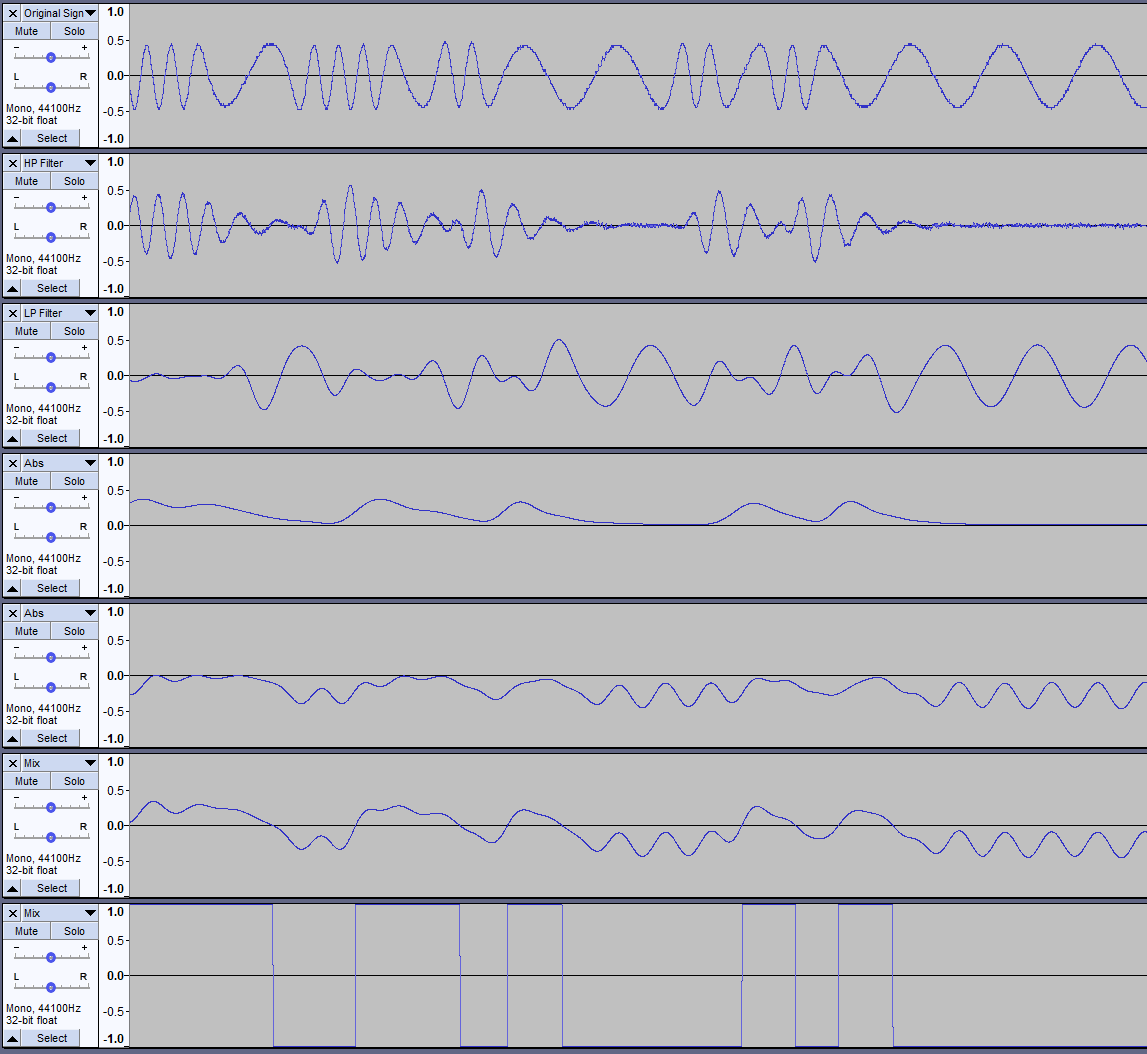
\includegraphics[width=\textwidth]{images/6-pentesting/audacity-demodulation.png}
    \caption{The process of demodulating an FSK signal in Audacity.}
    \label{fig:audacity-demodulation}
\end{figure}
This process was applied to all captured signals. However, the result of this process is a binary wave, not the actual binary data. To extract the binary data a simple python program was created, see figure \todo.

\subsection{Results}
\todo

\subsection{Discussion}
\todo
